\chapter{Desarrollo}

	A continuaci\'on se describe de forma detallada, el diseño y desarrollo del paquete para la clasificaci\'on de tub\'erculos de papa criolla(\textit{Solanum phureja}) para diferentes densidades de siembra empleando redes neuronales probabil\'isticas (apnnClassifier), siguiendo la metodolog\'ia descrita en el cap\'itulo 3.
	
\section{Creación del esqueleto del paquete.}
	
	Para esta fase se utilizó el ambiente de desarrollo RStudio, el cual es un entorno de desarrollo integrado de fuente abierta para R que agrega muchas caracter\'isticas y herramientas de productividad, además de facilitar el uso de R integrando la ayuda y la documentación.\\
En esta primera etapa se creó la estructura del paquete, la cual esta conformada por la identificación por nombre y descripción del paquete(Figura 4.1), además, se cargan los paquetes del CRAN de R y sus extensiones, de los cuales dependen los metodos y funciones que permitiran el desarrollo del paquete apnnClassifier; los mismos fueron almacenados en el repositorio local que se crea para este paquete durante el proceso de desarrollo; los principales fueron:\\

\begin{itemize}
\item plotly(Carson, S. \textit{et. al}, 2018; https://cran.r-project.org/web/packages/plotly/index.html)
\item readxl(Wickham, H. \textit{et. al}, 2018; https://cran.r-project.org/web/packages/readxl/index.html)
\item corrplot(Wei, T. \textit{et. al}, 2017; https://cran.r-project.org/web/packages/corrplot/index.html)
\item psych(Revelle, W. \textit{et. al}, 2019; https://cran.r-project.org/web/packages/psych/index.html)
\item spdep(Bivand, R. \textit{et. al}, 2018; https://cran.r-project.org/web/packages/spdep/index.html)
\item RCurl(Duncan Temple Lang and the CRAN team, 2018; https://cran.r-project.org/web/packages/RCurl/index.html)
\end{itemize}

\begin{figure}[h]
	\caption{Descripción del paquete}
	\centering
	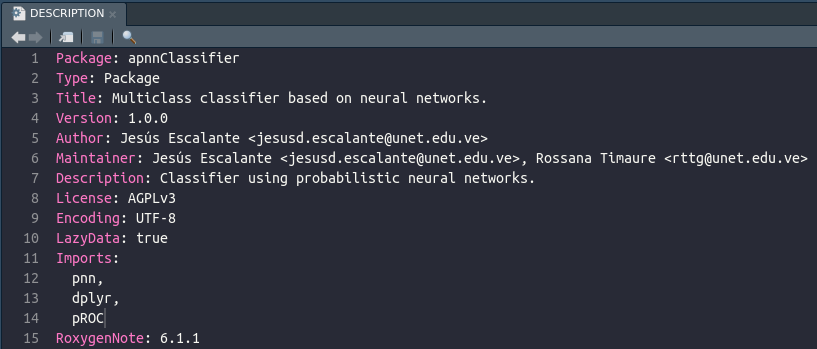
\includegraphics[scale=0.5]{package-description.png}
	\label{fig:arch}
\end{figure}

